\section{Project idea}
The idea for this project is to create a game using augmented reality (AR). 
Two teams will compete against each other to score the most goals using a ball. 
Each player will be equipped with a Google Cardboard, and these will display the playing field from a top-down 2D view. 
To achieve this, each player's position needs to be tracked as well as where the ball is located on the field.
In the top down view each player needs to see the positions of the other players and the ball.
They also need to see their own position on the playing field and where the goalposts are.
The players should be able to set an amount of goals they need to score to win before beginning the game. 
\begin{figure}[H]
    \centering
    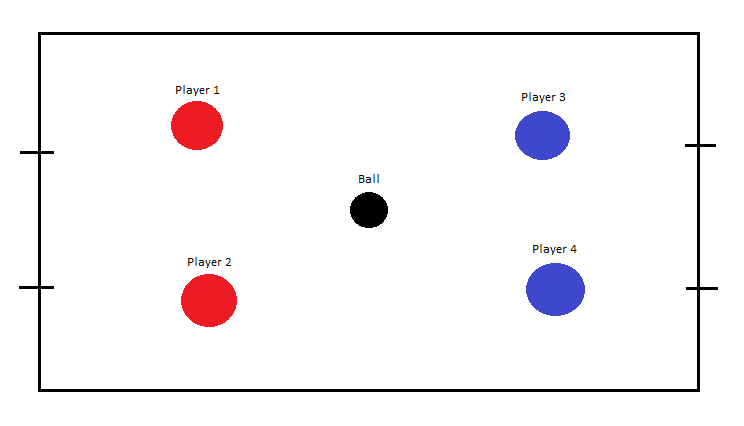
\includegraphics[width=0.6\linewidth]{Spil.PNG}
    \caption{An illustration of the playing field}
    \label{fig:game_illustration}
\end{figure}
In \autoref{fig:game_illustration}, an illustration of the playing field for the game is shown.
There are goalposts in each end of the field, and the teams score goals by getting the ball between the goalposts.
There could also be another version of the game where, instead of goalposts, there are goal zones into which the teams need to bring the ball.
These zones could even change locations as the game progressed.
\subsection{Problems to consider}
The project idea proposes some problems that will need to be solved for the game to work.
We will need to consider which technology we should be using to develop the augmented reality part of the game which shows the top-down view for each player. 
As it is something we do not have experience with, it would be preferable if we do not have to build it from scratch.
We will also need hardware that is able to track the positions of players and the ball.
This must be accurate and update quickly such that the players do not run into each other, otherwise the game will not work.
Another problem to consider is how the ball should be displayed in a 2D view.
For the players to be able to find the ball on the field, it either has to be quite large to make it easier to find from the top-down view, or the game will need some metric to display how far the ball is from the ground.
The game will also need to be able to track when the ball has crossed the goalline and then give feedback to the players.
Another problem to solve is how to keep the positional data synchronized across all the players' devices, as it will be difficult to play the game without accurate data.
